\chapter{Unstructured mesh Generation using Gmsh}
\thispagestyle{empty}
\label{sec:chap18}
\newcommand{\LocCHoneeightfig}{\Origin/CHAPTERS/chap18/figures}

In the previous chapter we saw how to create a Sphere in Gmsh. This chapter is a continuation of the last chapter and it is expected that the user has practiced and gone through it. Gmsh being a finite element mesh generator can be used to generate unstructured mesh (tri, prisims, etc). Since mesh generation is an important step in CFD simulation, we will look into the steps required to generate unstructured meshes and also make some changes in the geometry (.geo) file of Gmsh.

\section{Geometry}

Flow over a sphere has a vast engineering application. These simulations provide a test of the ability of the code to accurately reproduce typical flow structures observed in generic bluff body flows, such as those experienced by submarines and Unmanned Underwater Vehicles (UUVs). The geometry setup for our case is as shown in the Fig \ref{geom} below. We can see that the right left side of the geometry is termed as Inlet and the right side is termed as outlet which shows that the flow will move from left to right. The remaining sides of the geometry such as the top, bottom and side wslls are kept as empty. Sphere is fixed at the center of the domain. Length of the domain is 45 x 45 x 30 (L x B x H ) and radius of the sphere is 1 (Chapter 17). We have used this as an example in this chapter and actual dimensions can vary from case to case.
    
\begin{figure}[h]  
\centering
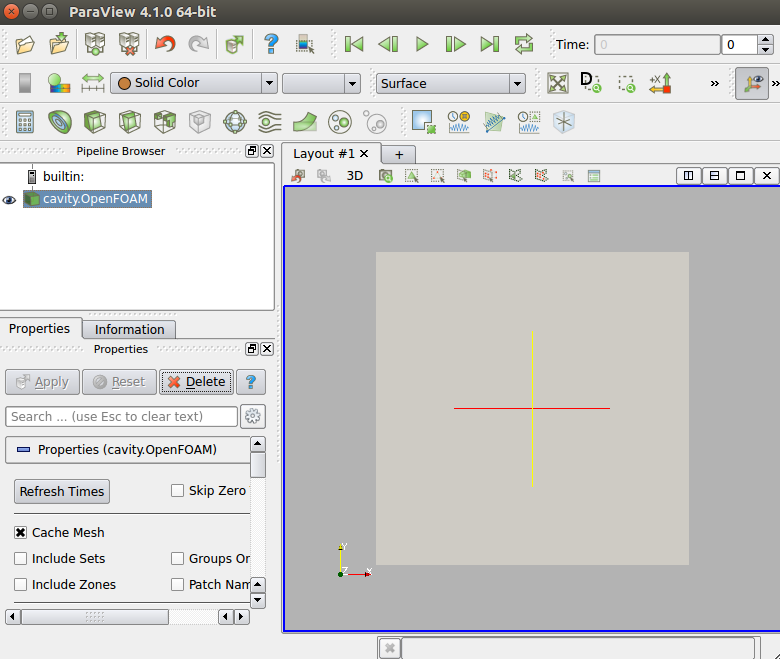
\includegraphics[scale=0.35]{\LocCHoneeightfig/geom.png}
\caption{Geometry for mesh generation}
\label{geom}
\end{figure}
    
\section{Creating Domain}

We need to create domain around the sphere as seen in the Fig \ref{geom}. Use the Geometry module in Gmsh to generate points (Chapter 16). Since it is a 3 Dimensional geometry we have eight points in our domain as given below,

\begin{itemize}
  \item (-15 ,-15 ,-15)
  \item (-15 , 15 ,-15)
  \item (-15 ,-15 , 15)
  \item (-15 , 15 , 15)
  \item ( 30 ,-15 ,-15)
  \item ( 30 , 15 ,-15)
  \item ( 30 ,-15 , 15)
  \item ( 30 , 15 , 15)
\end{itemize}

\flushleft Join all these points using lines (Straight Line) option under points. The final geometry will be as shown in Fig \ref{final-geom}.

\begin{figure}[h]  
\centering
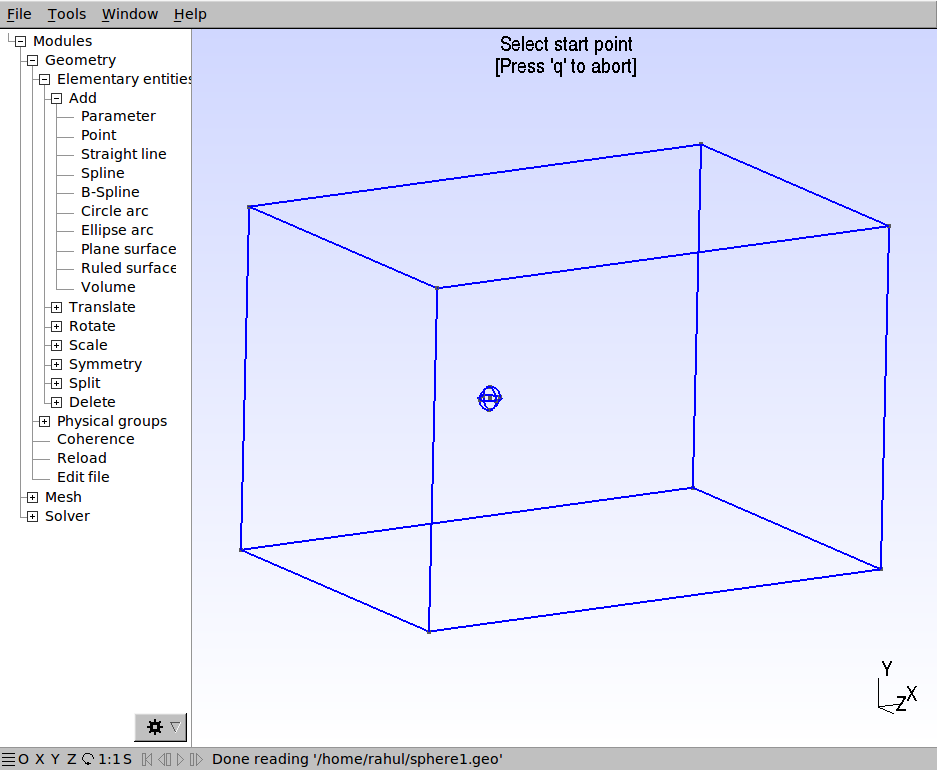
\includegraphics[scale=0.35]{\LocCHoneeightfig/final.png}
\caption{Creating and joining points}
\label{final-geom}
\end{figure}

\section{Surface and Volume}

We will now create surface for the geometry. Note that in this case we are using the option Plane surface instead of Ruled Surface. The difference between the two is that Ruled surface is used for creating a surface that can be interpolated using transfinite interpolation i.e. Sphere and a Plane Surface can be used for creating a planar surface. Now select four edges of a face, as we had seen in the previous chapter these edges turn red in Color upon selection, Fig \ref{surf}. After we select the four edges press e to end selection and q to abort. Repeat this process for the remaining faces. Once the a surface is created you notice a dotted crossed line, Fig \ref{surf1}.

\begin{figure}[h]  
\centering
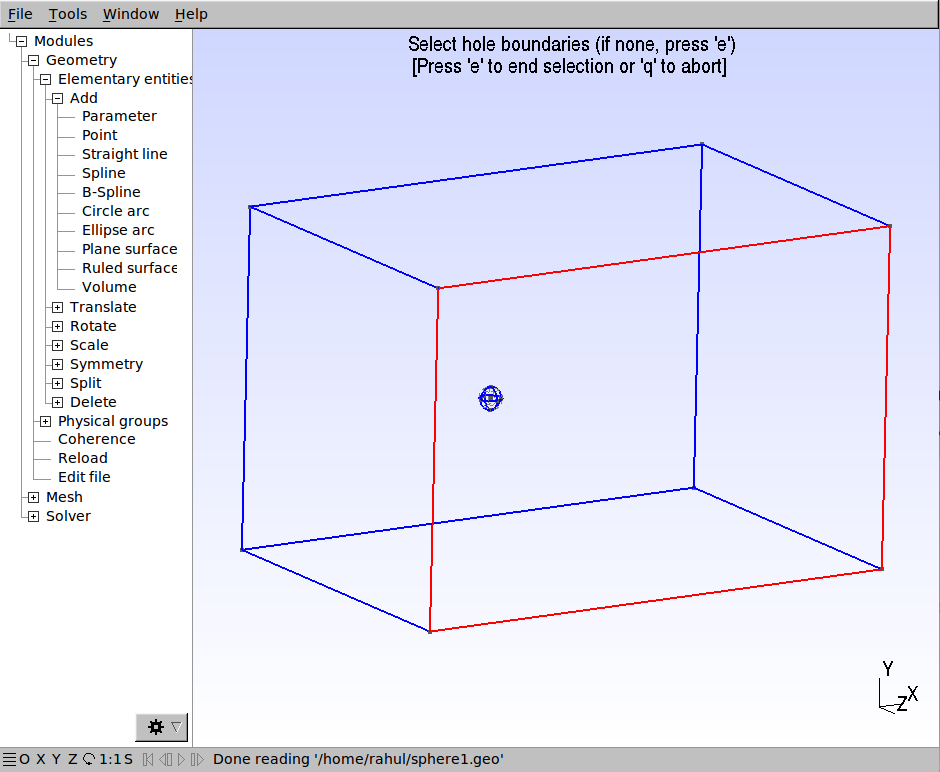
\includegraphics[scale=0.35]{\LocCHoneeightfig/surf.png}
\caption{Surface Selection}
\label{surf}
\end{figure}

\begin{figure}[h]  
\centering
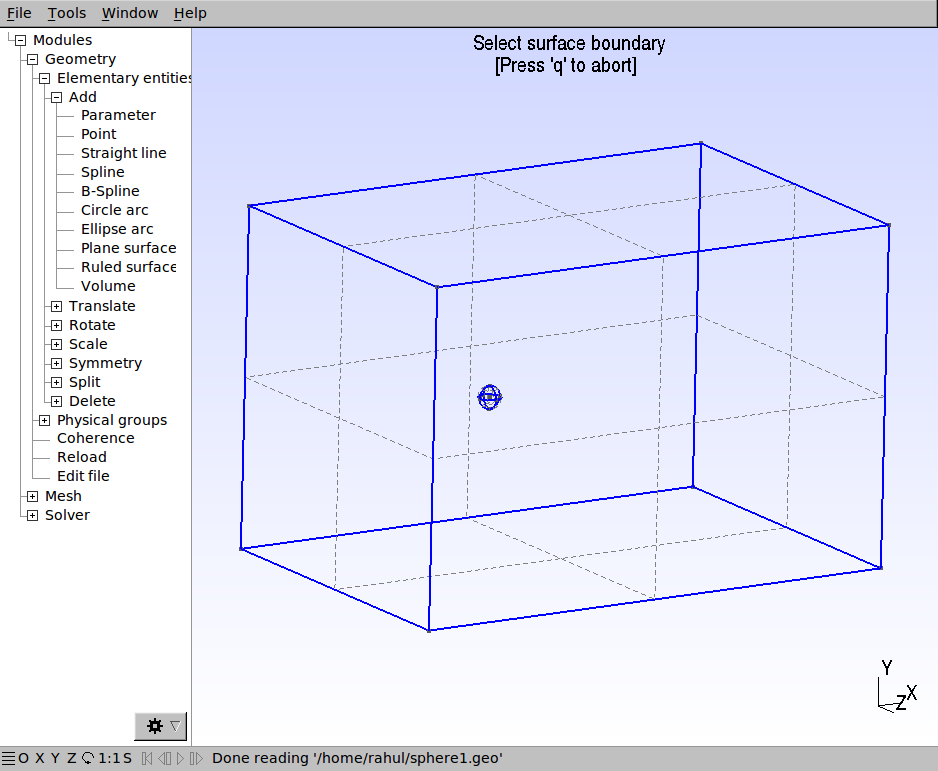
\includegraphics[scale=0.35]{\LocCHoneeightfig/surf1.png}
\caption{Surface Creation}
\label{surf1}
\end{figure}

\subsection{Physical Groups}

The purpose of physical entities is to assemble elementary entities into larger, possibly overlapping groups, and to control the orientation of the elements in these groups.
Since we require boundary names in our mesh file we group the faces under one commom name.\\

\flushleft Go to Physical Surface > Add > Surface and select a surface according to the boundary names given in the Geometry setup. Select the left face first since it is the Inlet, Fig \ref {inlet} and press e to end selection. Now click on the right face for outlet, Fig \ref{out} and press e to end selection. The remaining sides of the geometry are walls, so select all the four sides, Fig \ref{wall} and press e to end selection.

\begin{figure}[h]  
\centering
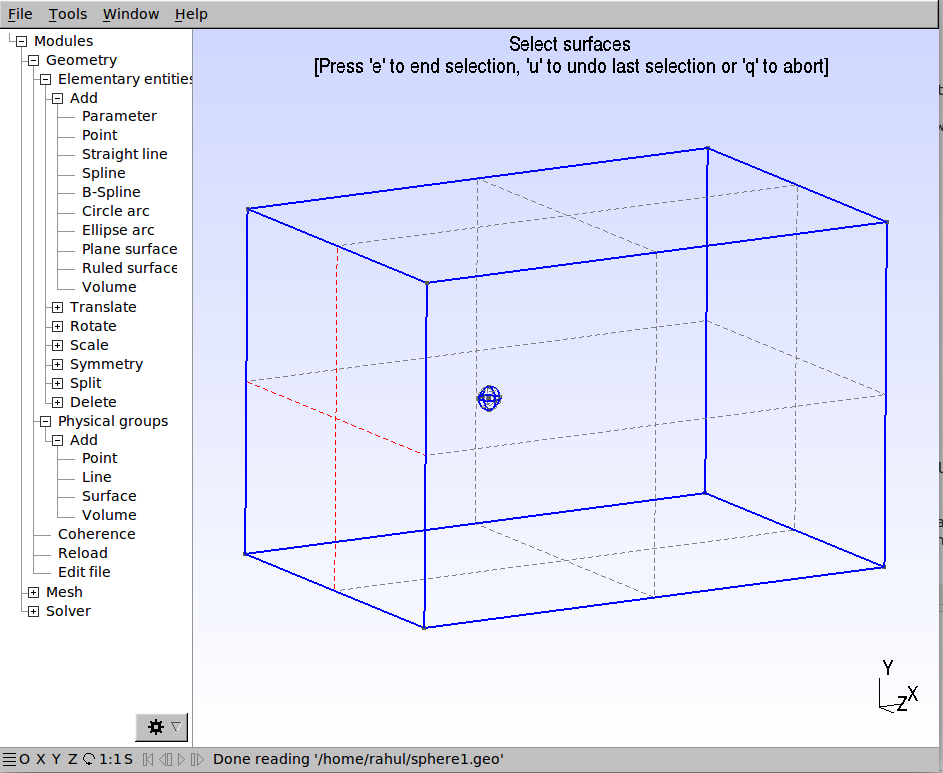
\includegraphics[scale=0.35]{\LocCHoneeightfig/inlet.png}
\caption{Physical Groups : Inlet}
\label{inlet}
\end{figure}

\begin{figure}[h]  
\centering
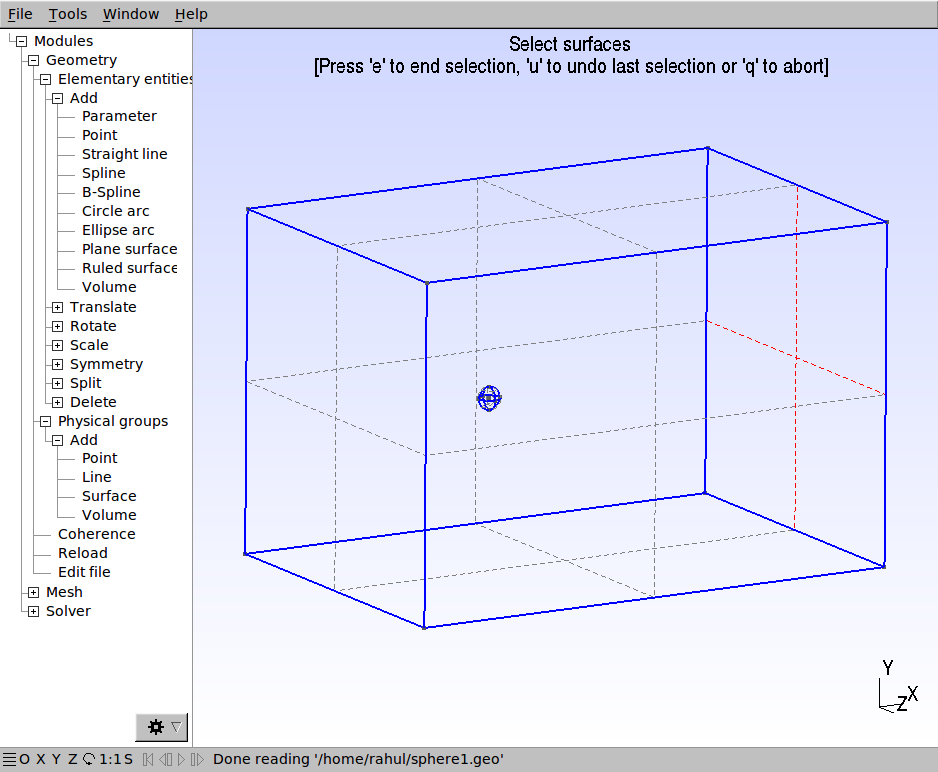
\includegraphics[scale=0.35]{\LocCHoneeightfig/out.png}
\caption{Physical Groups : Outlet}
\label{out}
\end{figure}

\begin{figure}[h]  
\centering
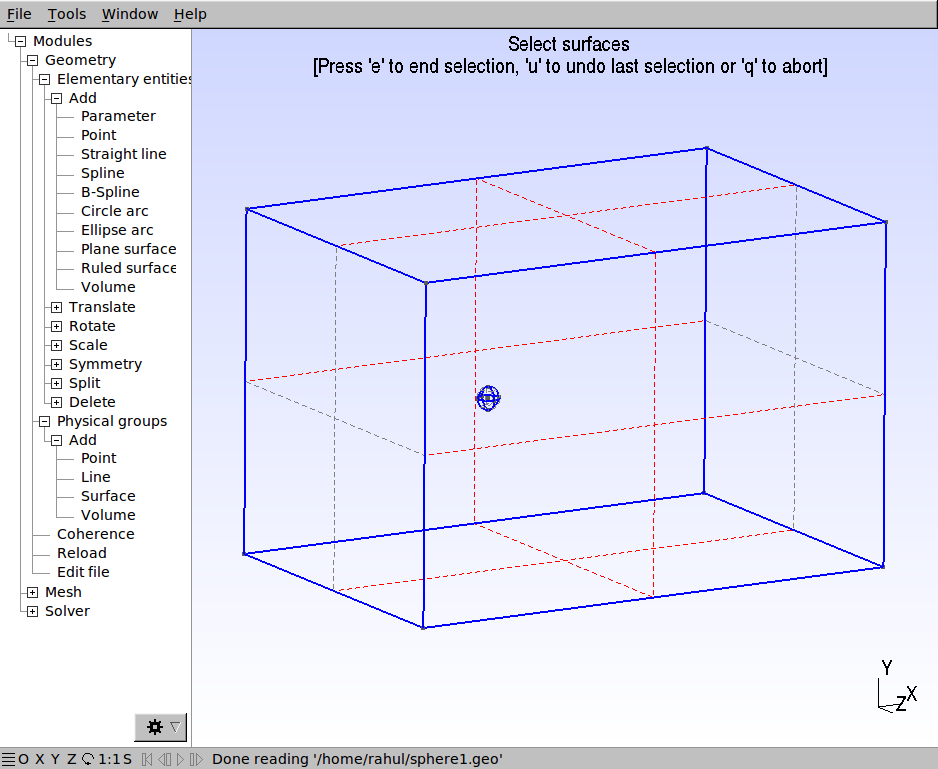
\includegraphics[scale=0.35]{\LocCHoneeightfig/walls.png}
\caption{Physical Groups : Walls}
\label{wall}
\end{figure}

\flushleft Since we are working on the same geometry file (Sphere1.geo) we will now open this file in a text editor. Note that there are new points added here. Also the Identification number for the entities are in continuation of the earlier series eg, In the .geo file on top we can see Points along with its Identification number 7. Now the new Point created has an Identification Number 8. As we had seen in the earlier chapter we can change the mesh element size, change the last variable in Points from 1 to d as shown below for all the points from 8 to 15 and at the beginning of the file type d = 0.5 and end it with a semi-colon.

\begin{itemize}
  \item Point(8) = {-15, -15, -15, d};
\end{itemize}

\flushleft Now we need to name the Physical Surfaces we created earlier. We need to replace the Identification number for the Surface under Physical Surfaces (54) to desired name of our boundary as shown below. It is important to keep in mind the order in which we selected the faces here, since that will be the boudnary name for that particular face when we export the file in OpenFOAM. As we had selected the first face as the left face we will name it as Inlet.

\begin{itemize}
  \item Physical Surface ("Inlet") = {51};
\end{itemize}

Replace the Identification number by the Boundary name "Inlet", do not forget to use these double quotes. Repeat this for Outlet and Walls.

\subsection{Volume}

To define the Volume we need to build surfaces, for this one has to define surface loops. In the .geo file now at the bottom of the file type,

\begin{itemize}
  \item Surface Loop() = {};
\end{itemize}

\flushleft In round brackets Identification number is the next integer after the Identification number in Physical Surface, In my case it is 63. In the currly brackets enter the ID's of the Plane Surface, in our case we have 6 faces and hence 6 ID's. The Surface Loop will be as shown below,

\begin{itemize}
  \item Surface Loop(63) = {49, 51, 53, 55, 57, 59};
\end{itemize}

\flushleft After we define the Surface Loop we can now create Volume for th mesh. Type this line after the Surface Loop as shown below,

\begin{itemize}
  \item Volume() = {};
\end{itemize}

\flushleft Inside the round brackets enter 64 as the next Identification number after 63 in Surface Loop. Since we have two volumes in our geometry i.e Sphere and the Rectangular domain we will enter the respective Surface Loop ID's here as shown below.

\begin{itemize}
  \item Volume(64) = {36, 63};
\end{itemize}

Finally we need to create a Physical Volume. To do this in the next line under Volume type the Line given below,

\begin{itemize}
  \item Physical Volume()={};
\end{itemize} 

\flushleft Under round brackets enter 65 as the next Identification number after 64 in Volume. On the right hand side under curely brackets enter the Identification Number for Volume i.e 64. Our file is now ready, we can save it and close.

\begin{itemize}
  \item Physical Volume(65)={64};
\end{itemize}

\section{Meshing}

Now in Gmsh open the geometry file (Sphere1.geo) that we just saved. Gmsh follows a bottom to top approach for meshing i.e first we start with 1D meshing for meshing the edges of the geometry. Followed by 2D meshing for surfaces and Finally 3D Meshing for Volume. You can either mesh the geometry using the Mesh module in Gmsh or using F1 key for 1D meshing, F2 for 2D meshing and F3 key for 3D Meshing. We will now select F1 key for 1D meshing, we can see the message in the console below stating that 1D meshing is done, Fig \ref(1d). Now press F2 key for 2D meshing, Fig \ref{2d} and Finally press F3 key for 3D mehsing, Fig\ref{3d}.

\begin{figure}[h]  
\centering
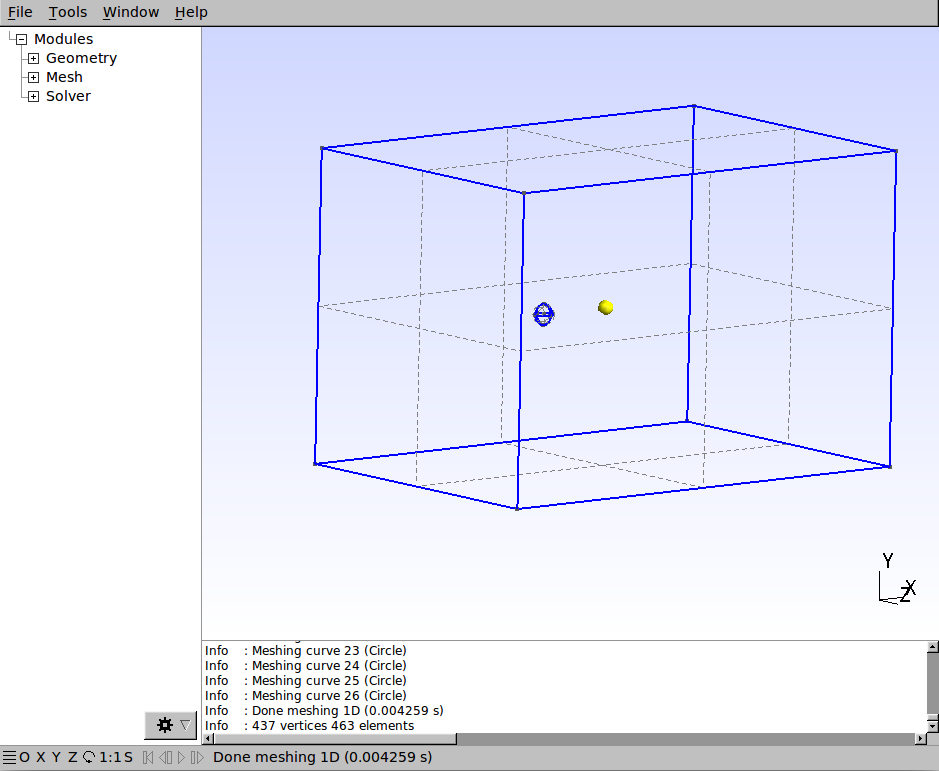
\includegraphics[scale=0.35]{\LocCHoneeightfig/1d.png}
\caption{One Dimensional Meshing}
\label{wall}
\end{figure}

\begin{figure}[h]  
\centering
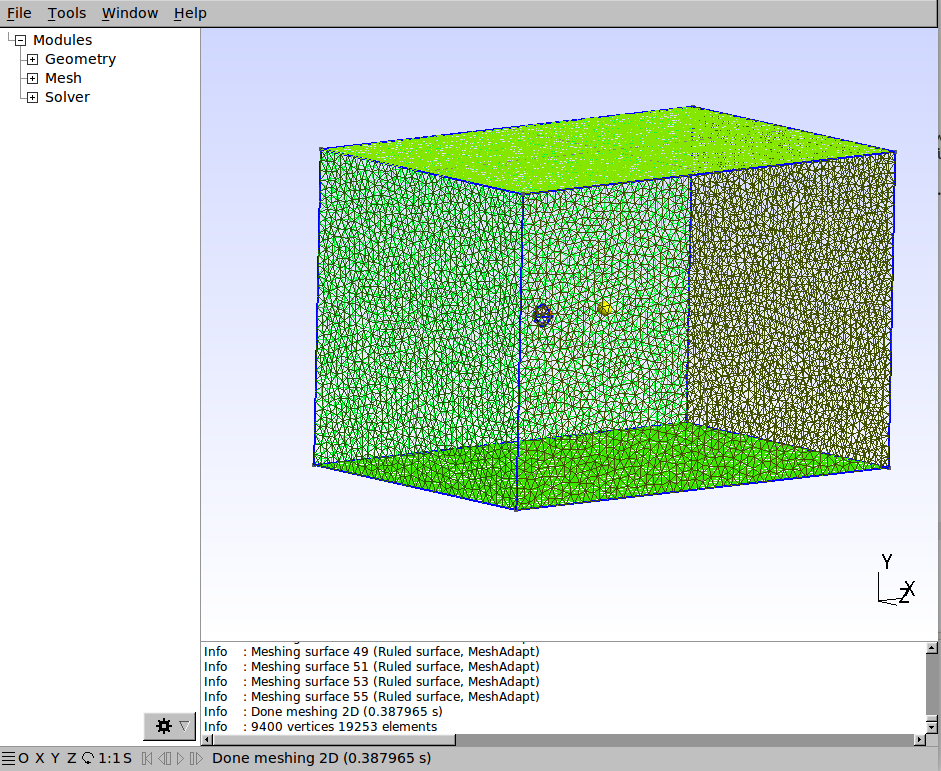
\includegraphics[scale=0.35]{\LocCHoneeightfig/2d.png}
\caption{Two Dimensional Meshing - Surface }
\label{wall}
\end{figure}


\begin{figure}[h]  
\centering
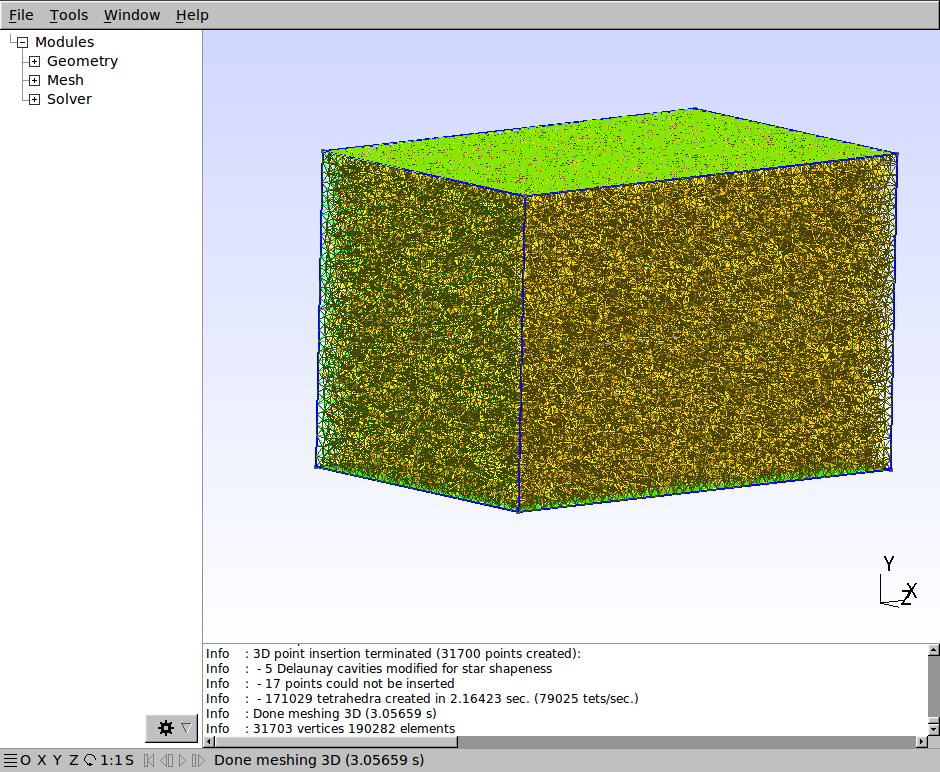
\includegraphics[scale=0.35]{\LocCHoneeightfig/3d.png}
\caption{Three Dimensional Meshing - Volume}
\label{wall}
\end{figure}

\flushleft We can also optimize the mesh using the Optimize funtions available under the mesh module. Click on the Optimize 3D netgen option.
